% ============================ SCHEDULE ==================================
\phase{Phase three \textbullet\ When}{The schedule, and the deadline hiding inside it}{A work breakdown, a critical path, 50,000 simulated timelines, and a policy cliff on 31 December 2030.}\label{sec:schedule}

\subsection{Breaking the work down}
A work breakdown structure (WBS) splits the project into packages small enough to cost, schedule and give to one owner. Ours has six branches.

\begin{figure}[H]
\centering
\begin{tikzpicture}[
  top/.style={rounded corners=2pt,fill=ink,text=paper,font=\footnotesize\bfseries,align=center,inner sep=4pt},
  l1/.style={rounded corners=2pt,draw=audit,line width=0.6pt,fill=paper,font=\scriptsize\bfseries,align=center,text width=19mm,inner sep=3pt,minimum height=9mm},
  l2/.style={font=\scriptsize,align=left,text width=19mm,anchor=north},
  edge/.style={draw=ink2,line width=0.5pt}]
\node[top] (r) at (0,0) {Paradip Green Hydrogen Phase 1 (100 MW)};
\foreach \i/\t/\items in {
  0/{1.0 Development}/{1.1 Site study (A)\\1.2 Land, consents, PESO (C)\\1.3 FEED, Class 3 cost (D)},
  1/{2.0 Commercial}/{2.1 Offtake contract (B)\\2.2 Power purchase\\2.3 Insurance},
  2/{3.0 Finance}/{3.1 Lender due diligence\\3.2 Financial close (E)\\3.3 Hedging},
  3/{4.0 Procurement}/{4.1 Alkaline 80 MW (F)\\4.2 PEM 20 MW (G)\\4.3 Transformers, rectifiers (H)},
  4/{5.0 Construction}/{5.1 Civil works (I)\\5.2 Mechanical, integration (K)\\5.3 Pipeline to refinery},
  5/{6.0 Grid and start-up}/{6.1 CTU connectivity (J)\\6.2 Commissioning (L)\\6.3 Certification}}{
  \node[l1] (n\i) at (\i*22mm-55mm,-15mm) {\t};
  \node[l2] at (\i*22mm-55mm,-21mm) {\items};
  \draw[edge] (r.south) -- ++(0,-3.5mm) -| (n\i.north);}
\end{tikzpicture}
\caption{Work breakdown structure. Letters in brackets link each package to an activity in the schedule network.}
\end{figure}

\subsection{The network and the critical path}
Each activity has three duration estimates: optimistic, most likely and pessimistic. Lead times for transformers and electrolysers follow what Dossier 1 found in the market; the grid connection (J) gets the widest range because it is the task developers complain about most \cite{gemini2026}. \estd

\begin{center}\tablefont
\begin{tabularx}{\textwidth}{@{}c L c c c c c@{}}
\toprule
\thead{ID} & \thead{Activity} & \thead{Months (o/m/p)} & \thead{Needs} & \thead{PERT mean} & \thead{Slack} & \thead{Critical in}\\ \midrule
A & Pre-feasibility and site selection & 3 / 4 / 6 & -- & 4.2 & 0 & 100\%\\
B & Offtake negotiation, 25-year contract & 6 / 9 / 15 & A & 9.5 & 0 & 46\%\\
C & Land, consents, PESO approvals & 6 / 9 / 14 & A & 9.3 & 0 & 41\%\\
D & FEED to AACE Class 3 estimate \cite{epcland} & 6 / 8 / 12 & A & 8.3 & 1 & 13\%\\
E & Financing and financial close (FID) & 3 / 5 / 9 & B, C, D & 5.3 & 0 & 100\%\\
F & Alkaline electrolysers, 80 MW & 10 / 14 / 20 & E & 14.3 & 0 & 45\%\\
G & PEM electrolysers, 20 MW & 8 / 11 / 16 & E & 11.3 & 3 & 3\%\\
H & Transformers and rectifiers & 10 / 14 / 22 & E & 14.7 & 0 & \textbf{52\%}\\
I & Civil works and site preparation & 8 / 10 / 14 & E & 10.3 & 4 & 0.3\%\\
J & RE contracts and CTU connectivity & 12 / 18 / 30 & B & 19.0 & 9 & 0.3\%\\
K & Mechanical installation, integration & 6 / 8 / 12 & F, G, H, I & 8.3 & 0 & 100\%\\
L & Commissioning, performance tests & 3 / 4 / 7 & K, J & 4.3 & 0 & 100\%\\
\bottomrule
\end{tabularx}
\end{center}

Using the most-likely durations, the critical path (the longest chain, where any delay delays the whole project) runs \textbf{A $\rightarrow$ B/C $\rightarrow$ E $\rightarrow$ F/H $\rightarrow$ K $\rightarrow$ L} and finishes in \textbf{44 months}. Several branches tie, which is the first warning sign.

\begin{figure}[H]
\centering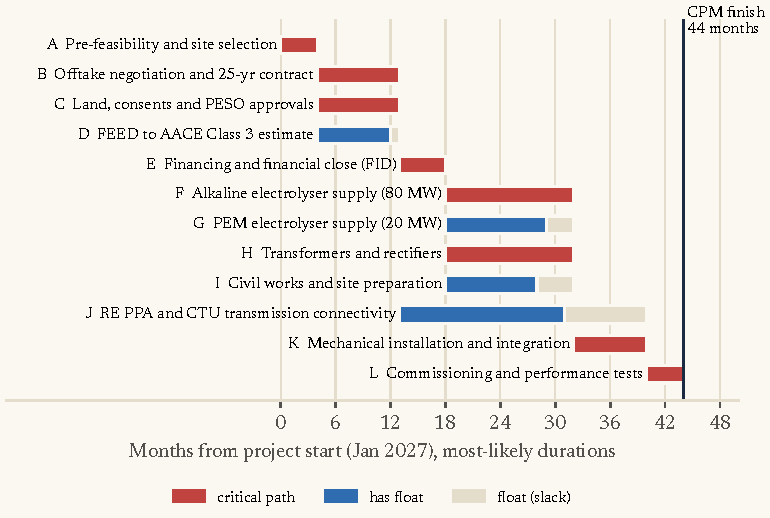
\includegraphics[width=\textwidth]{gantt.pdf}
\caption{Gantt chart at most-likely durations. Red bars are critical; grey shows float. Source: \texttt{schedule.py}.}
\end{figure}

\subsection{Why the plan will probably run late: merge bias}
The classic PERT method adds up the expected durations along one path \cite{malcolm1959}. It quietly assumes only one path can be late. In a network where several paths meet at one point (here, at financial close E and at installation K), the project waits for the \emph{slowest} of them, and the slowest of several uncertain things is later, on average, than any one of them. This is called merge bias, and it was spotted only five years after PERT was invented \cite{maccrimmon1964}.

So we simulated the project 50,000 times, drawing every duration from a Beta-PERT distribution.

\begin{figure}[H]
\centering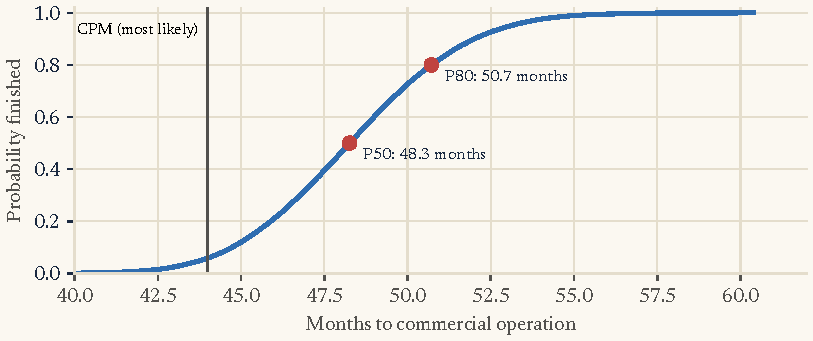
\includegraphics[width=\textwidth]{schedule_mc.pdf}
\caption{Distribution of completion times across 50,000 simulated projects. Source: \texttt{schedule.py}.}
\end{figure}

\begin{center}\tablefont
\begin{tabularx}{0.86\textwidth}{@{}L c@{}}
\toprule
\thead{Measure} & \thead{Months from January 2027}\\ \midrule
Critical-path plan (most likely durations) & 44.0\\
P50 (half the simulated projects finish by then) & 48.3\\
P80 (the date we would promise a lender) & 50.7\\
P90 & 52.0\\
Merge bias (P50 minus plan) & +4.3\\
\bottomrule
\end{tabularx}
\end{center}

\begin{finding}[The long pole is the transformer, not the electrolyser]
Across the simulations, the transformers and rectifiers (H) lie on the critical path 52\% of the time; the alkaline stacks (F) 45\%. Grid-scale transformers have become a global bottleneck because every renewable and data-centre project wants them at once. A project manager who watches only the electrolyser order is watching the wrong machine. \confM
\end{finding}

\subsection{The deadline hiding inside the schedule}
India waives inter-state transmission charges for 25 years for green hydrogen plants commissioned by \textbf{31 December 2030} \cite{sq2023ists} \rep. Starting in January 2027, that date is month 48. Our P50 is month 48.3.

\begin{verdict}[The schedule is a finance problem]
\textbf{As planned, the plant has only a 46\% chance of being commissioned before the transmission waiver closes.} Missing it would add a transmission charge to every unit of power we buy for 25 years. If that charge were even ₹0.40/kWh, the price we need would rise by about ₹23/kg (each \usd{}1/MWh of power costs about ₹5.3/kg in our model) \estd\ \confL\ (for the size of the charge).
\end{verdict}

\noindent What we can do about it, tested in the model:
\begin{itemize}
\item \textbf{Release long-lead orders before financial close.} A ``limited notice to proceed'' lets the transformer and electrolyser makers start work three months before the loan is signed, with a reservation payment at risk. That lifts the chance of meeting the deadline from \textbf{46\% to 82\%} (two months: 72\%; four months: 89\%) and pulls the P80 to month 47.8. The deposit, perhaps 10\% of the electrolyser order (about ₹75 crore), is lost only if the project dies before close. The 36-point gain in probability, against a waiver worth on the order of ₹200 crore in present value, is worth about ₹70 crore; the bet is favourable as long as the chance of the project dying after the deposit is low. \estd
\item \textbf{Run land and offtake in parallel with a time box.} B and C are each critical about 40--46\% of the time; neither can be allowed to drift.
\item \textbf{Put P80, not the plan, in the contracts.} The buyer and lenders get month 51 as the guaranteed date, with liquidated damages from the EPC contractor for every week late beyond that.
\end{itemize}

\begin{plainwords}[Earned value: how we will track it]
Once construction starts we report three numbers each month: what we planned to have done (planned value), what we have actually done (earned value) and what it cost (actual cost). Two ratios fall out. The schedule performance index (earned over planned) tells us whether we are ahead or behind; the cost performance index (earned over actual) tells us whether we are getting a rupee of work for each rupee spent. An index below 0.95 for two months running goes to the steering committee.
\end{plainwords}
\newpage
